\documentclass[]{article}
\usepackage[T1]{fontenc}
\usepackage[english]{babel}
\usepackage[utf8]{inputenc}
\usepackage{color}
\usepackage{listings}
\usepackage{courier}
\usepackage{cite}
\usepackage{graphicx}
\usepackage{hyperref}
\usepackage[xindy]{glossaries}
\makeglossaries

\newacronym{dac}{DAC}{Discretionary Access Control}
\newacronym{mac}{MAC}{Mandatory Access Control}
\newacronym{nsa}{NSA}{National Security Agency}
\newacronym{sel}{SELinux}{Security-Enhanced Linux}
\newacronym{dte}{DTE}{Domain and Type Enforcement}
\newacronym{lids}{LIDS}{Linux Intrusion Detection System}
\newacronym{lsm}{LSM}{Linux Security Modules}

\lstset{ %
language=C,                % choose the language of the code
basicstyle=\footnotesize\ttfamily,       % the size of the fonts that are used for the code
numbers=left,                   % where to put the line-numbers
numberstyle=\footnotesize,      % the size of the fonts that are used for the line-numbers
stepnumber=1,                   % the step between two line-numbers. If it is 1 each line will be numbered
numbersep=5pt,                  % how far the line-numbers are from the code
backgroundcolor=\color{white},  % choose the background color. You must add \usepackage{color}
showspaces=false,               % show spaces adding particular underscores
showstringspaces=false,         % underline spaces within strings
showtabs=false,                 % show tabs within strings adding particular underscores
frame=bt,           % adds a frame around the code
tabsize=2,          % sets default tabsize to 2 spaces
captionpos=b,           % sets the caption-position to bottom
breaklines=true,        % sets automatic line breaking
breakatwhitespace=false,    % sets if automatic breaks should only happen at whitespace
escapeinside={\%*}{*)}          % if you want to add a comment within your code
}


\begin{document}

\title{Introduction to Linux Security Modules}
%\subtitle{}
\author{Rui Gonçalo
        \\{\scriptsize \texttt{pg18378@alunos.uminho.pt}}
       }
\date{\today}
\maketitle

\begin{abstract}
``If you cannot explain it simply, you do not understand it well enough.''
\end{abstract}


\section{Introduction}

In 2001, Peter Loscocco and Stephen Smalley wrote an article introducing the \textit{\gls{sel}} \cite{LS01}. The main reason that led to the development of such mechanism was the flawed assumption that adequate security should reside in applications, leaving the role of the operating system behind \cite{LSMTTF98}. In fact, secure applications require secure operating systems. A strong concept related to operating systems security is \textit{access control policy}. This specifies which of the operations associated with an object are authorized to perform. Linux kernel inherited from the UNIX security model the \textit{\gls{dac}} that allows the owner of an object to set the security policy for that object (the control of access is based on the discretion of the owner). However, this model of access control brings some advantages. For instance, every program executed by a certain user receives all of the privileges associated with that user, and so it is able to change the permissions with all user's objects. In this sense, a \textit{\gls{mac}} was purposed to protect the system against vulnerabilities left by other access control models. In \gls{mac} the operating system constrains the ability of a subject to perform an operation on an object, depending on the security attributes. Whenever a subject attempts to access an object, an authorization rule enforced by the operating system kernel checks these security attributes in order to allow or deny the access.\\

\noindent
At the Linux Kernel 2.5 Summit, the \gls{nsa}, based on the security issues previously mentioned, presented their work on \gls{sel}, a security mechanism of a flexible access control architecture in the Linux kernel. \gls{nsa} reiterated the need for such support in the mainstream Linux kernel. Other projects were presented to enforce access policies, namely \gls{dte}, \gls{lids} and POSIX.1e capabilities. Given these projects, Linus Torvalds decided to provide a general framework for security policy, named \gls{lsm}. This framework allow many different access control models to be implemented as loadable kernel modules. Linus enforced that \gls{lsm} should be truly generic, where using a different security model was a question of loading a different kernel module. Should also be conceptually simple, minimally invasive and efficient. At last, the mechanism should be able to support the POSIX.1e capabilities logic as an optional security module \cite{WCSMK02}.\\

\section{Design}

The basic abstraction of the \gls{lsm} interface is to intercede in the access to internal kernel objects. Security modules should answer a simple question "May a subject \texttt{S} perform a kernel operation \texttt{OP} on an internal kernel object \texttt{OBJ}?". The mechanism that allow modules to execute this task lies in \textit{hook} functions that are placed in the kernel code, as shown in \autoref{fig:lsm_arch}.

\begin{figure}[htbp]
 \centering
 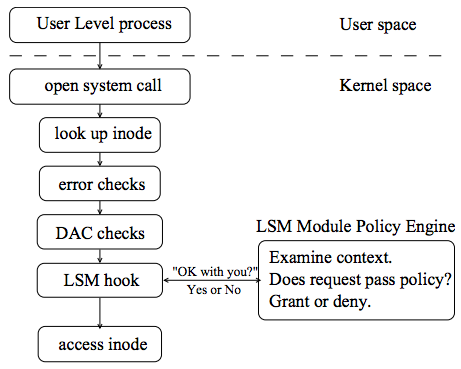
\includegraphics[scale=0.5]{images/LSM_architecture.png}
 \caption{LSM hook functions architecture}
 \label{fig:lsm_arch}
\end{figure}

Immediately before the kernel access the object, represented as \textit{inode} in \autoref{fig:lsm_arch}, the hook makes a call to a function that the \gls{lsm} module must provide. The module, based on policy rules, allow the access, or deny it, forcing an error code return.

\section{Implementation}

For a better understanding of the implementation of the \gls{lsm} framework it is important to take a look at the source code of the Linux kernel. \autoref{fig:kernel_arch} presents the relevant files in the kernel files hierarchy.   

\begin{figure}[htbp]
 \centering
 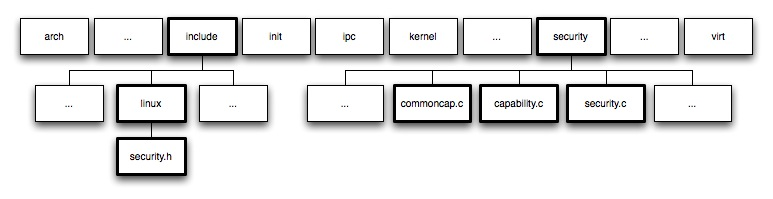
\includegraphics[scale=0.5]{images/kernel_arch.jpg}
 \caption{\gls{LSM} relevant files in the Linux kernel files hierarchy}
 \label{fig:kernel_arch}
\end{figure}

\subsection{Header file}

\noindent
The \texttt{include/linux/security.h} file contains the hook functions' declarations. The source code may be divided into two parts, depending on the value of the conditional group \texttt{CONFIG\_SECURITY} being true or false. In the first case, an extensive structure with pointers to all hook functions is declared. If false, only default functions are declared and the kernel loads the default security module. The code snippet in \autoref{lst:struct_ops}, extracted from the Linux kernel v3.11, presents the initial function pointers in the structure \texttt{security\_operations}.

\begin{lstlisting}[frame=none, numbers=none, caption=Security structure declaration (Linux kernel v3.11), label=lst:struct_ops]
struct security_operations {
	char name[SECURITY_NAME_MAX + 1];

	int (*ptrace_access_check) (struct task_struct *child, unsigned int mode);
	int (*ptrace_traceme) (struct task_struct *parent);
	int (*capget) (struct task_struct *target,
		       kernel_cap_t *effective,
		       kernel_cap_t *inheritable, kernel_cap_t *permitted);
	int (*capset) (struct cred *new,
		       const struct cred *old,
		       const kernel_cap_t *effective,
		       const kernel_cap_t *inheritable,
		       const kernel_cap_t *permitted);
	int (*capable) (const struct cred *cred, struct user_namespace *ns,
			int cap, int audit);
	int (*quotactl) (int cmds, int type, int id, struct super_block *sb);
	int (*quota_on) (struct dentry *dentry);
	int (*syslog) (int type);
	int (*settime) (const struct timespec *ts, const struct timezone *tz);
	int (*vm_enough_memory) (struct mm_struct *mm, long pages);
\end{lstlisting}

\noindent
Along with the structure, the functions' prototypes are declared, as shown in \autoref{lst:hooks}. Some security hooks are declared depending on conditional groups:

\begin{itemize}
 \item \texttt{CONFIG\_SECURITY\_PATH}, includes security hooks for pathname based access control;
 \item \texttt{CONFIG\_SECURITY\_NETWORK}, enables socket and network security hooks;
 \item \texttt{CONFIG\_SECURITY\_NETWORK\_XFRM}, security hooks for XFRM framework, that implement per-packet access controls based on labels derived from IPSec policy;
\item \texttt{CONFIG\_KEYS}, provides support for retaining authentication tokens and access keys in the kernel;
\item \texttt{CONFIG\_AUDIT}, enables auditing infrastructure that can be used with another kernel subsystem.
\end{itemize}

\begin{lstlisting}[frame=none, numbers=none, caption=Security hooks declaration, label=lst:hooks]
int security_ptrace_access_check(struct task_struct *child, unsigned int mode);
int security_ptrace_traceme(struct task_struct *parent);
int security_capget(struct task_struct *target,
		    kernel_cap_t *effective,
		    kernel_cap_t *inheritable,
		    kernel_cap_t *permitted);
int security_capset(struct cred *new, const struct cred *old,
		    const kernel_cap_t *effective,
		    const kernel_cap_t *inheritable,
		    const kernel_cap_t *permitted);
int security_capable(const struct cred *cred, struct user_namespace *ns,
			int cap);
int security_capable_noaudit(const struct cred *cred, struct user_namespace *ns,
			     int cap);
int security_quotactl(int cmds, int type, int id, struct super_block *sb);
int security_quota_on(struct dentry *dentry);
int security_syslog(int type);
int security_settime(const struct timespec *ts, const struct timezone *tz);
int security_vm_enough_memory_mm(struct mm_struct *mm, long pages);
\end{lstlisting}

\noindent
If the configurable option \texttt{CONFIG\_SECURITY} is not selected, the default security module is loaded. This module only executes a few capabilities, being permissive in all other hooks, which means that allow access to all kernel internal objects. \autoref{lst:default_hooks} exhibits some of these hooks' source code.

\begin{lstlisting}[frame=none, numbers=none, caption=Default security hooks' source code, label=lst:default_hooks]
static inline int security_capable(const struct cred *cred,
				   struct user_namespace *ns, int cap)
{
	return cap_capable(cred, ns, cap, SECURITY_CAP_AUDIT);
}

static inline int security_capable_noaudit(const struct cred *cred,
					   struct user_namespace *ns, int cap) {
	return cap_capable(cred, ns, cap, SECURITY_CAP_NOAUDIT);
}

static inline int security_quotactl(int cmds, int type, int id,
				     struct super_block *sb)
{
	return 0;
}

static inline int security_quota_on(struct dentry *dentry)
{
	return 0;
}

static inline int security_syslog(int type)
{
	return 0;
}
\end{lstlisting}

\noindent
The same process is kept to the other configurable options. Depending on their values, security hooks are either declared or coded with default instructions.

\subsection{Common capabilities}

Capabilities have always be a part of the Linux kernel. 

\renewcommand{\bibname}{References}
\bibliographystyle{ieeetr}
\bibliography{bibliography.bib}


\end{document}